\documentclass[tikz, border=10pt]{standalone}
\usetikzlibrary{shapes,fit}

\tikzset{
    pics/vhsplit/.style n args = {2}{
        code = {
        \draw [draw] (0,1) rectangle (1.25,0.5);
        \node[draw=none] at (0.625,0.75) {#1};
        \draw [draw] (1.25,1) rectangle (2,0.5);
        \node[draw=none] at (1.625,0.75) {#2};
        \draw [draw] (0,0.5) rectangle (1,0);
        \draw [draw] (1,0.5) rectangle (2,0);
        \node[draw=none] at (0.5,0.25) {\tiny{child}};
        \node[draw=none] at (1.5,0.25) {\tiny{next}};
        }
    }
}


\begin{document}
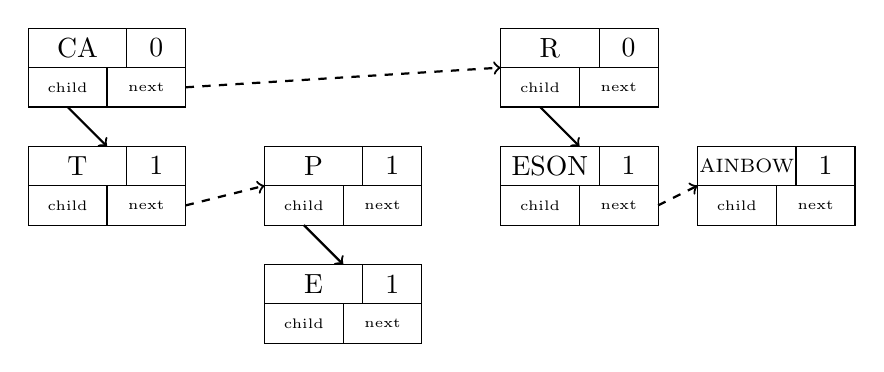
\begin{tikzpicture}%[every node/.append style={draw, rounded corners, inner sep=10pt}]
    %\path pic at (-3,0) {vhsplit={}{0}};
    %\coordinate(CAs) at (-2.5,0);

    \path pic at (-3,-1.5) {vhsplit={CA}{0}};
    %\coordinate(CAn) at (-2,-0.5);
    \coordinate(Rs) at (-1,-1.25);
    \coordinate(Ts) at (-2.5,-1.5);

    \path pic at (-3,-3) {vhsplit={T}{1}};
    \coordinate(Tn) at (-2,-2);
    \coordinate(Ps) at (-1,-2.75);

    \path pic at (0,-3) {vhsplit={P}{1}};
    \coordinate(Pn) at (0,-2.5);
    \coordinate(Es) at (0.5,-3);

    \path pic at (0,-4.5) {vhsplit={E}{1}};
    \coordinate(En) at (1,-3.5);

    %\draw [->,  thick] (CAs)--(CAn);
    \draw [->,  thick] (Ts)--(Tn);
    \draw [->,  thick, dashed] (Ps)--(Pn);
    \draw [->,  thick] (Es)--(En);

    \path pic at (3,-1.5) {vhsplit={R}{0}};
    \coordinate(Rn) at (3,-1);
    \coordinate(E1s) at (3.5,-1.5);

    \path pic at (5.5,-3) {vhsplit={\scriptsize{AINBOW}}{1}};
    \coordinate(A1n) at (5.5,-2.5);

    \path pic at (3,-3) {vhsplit={ESON}{1}};
    \coordinate(E1n) at (4,-2);
    \coordinate(A1s) at (5,-2.75);

    \draw [->,  thick, dashed] (Rs)--(Rn);
    \draw [->,  thick, dashed] (A1s)--(A1n);
    \draw [->,  thick] (E1s)--(E1n);

\end{tikzpicture}
\end{document}
